\documentclass[10pt, a4paper]{amsart}

\usepackage[]{graphicx}
\usepackage[]{hyperref}
\usepackage[]{physics}
\usepackage[]{listings}
\usepackage[T1]{fontenc}
\usepackage{color}

\definecolor{mygreen}{rgb}{0,0.6,0}
\definecolor{mygray}{rgb}{0.5,0.5,0.5}
\definecolor{mymauve}{rgb}{0.58,0,0.82}

\lstset{ %
  backgroundcolor=\color{white},   % choose the background color; you must add \usepackage{color} or \usepackage{xcolor}
  basicstyle=\footnotesize,        % the size of the fonts that are used for the code
  breakatwhitespace=false,         % sets if automatic breaks should only happen at whitespace
  breaklines=true,                 % sets automatic line breaking
  captionpos=b,                    % sets the caption-position to bottom
  commentstyle=\color{mygreen},    % comment style
  deletekeywords={...},            % if you want to delete keywords from the given language
  escapeinside={\%*}{*)},          % if you want to add LaTeX within your code
  extendedchars=true,              % lets you use non-ASCII characters; for 8-bits encodings only, does not work with UTF-8
  frame=single,	                   % adds a frame around the code
  keepspaces=true,                 % keeps spaces in text, useful for keeping indentation of code (possibly needs columns=flexible)
  keywordstyle=\color{blue},       % keyword style
  language=c++,                 % the language of the code
  otherkeywords={*,...},           % if you want to add more keywords to the set
  rulecolor=\color{black},         % if not set, the frame-color may be changed on line-breaks within not-black text (e.g. comments (green here))
  showspaces=false,                % show spaces everywhere adding particular underscores; it overrides 'showstringspaces'
  showstringspaces=false,          % underline spaces within strings only
  showtabs=false,                  % show tabs within strings adding particular underscores
  stepnumber=2,                    % the step between two line-numbers. If it's 1, each line will be numbered
  stringstyle=\color{mymauve},     % string literal style
  tabsize=2,	                   % sets default tabsize to 2 spaces
}

\title[Solving the Poisson-equation in one dimension]{Solving the Poisson-equation in one dimension: \\
\normalsize{TDMA vs LU} \\
  \hrulefill\small{ FYS3150: Computational Physics }\hrulefill}

\author[Svalheim \& Winther-Larsen]{Trygve Leithe Svalheim \\
   Sebastian G. Winther-Larsen \\
  \href{https://github.com/gregwinther/FYS3150/}{\texttt{github.com/gregwinther}}}

\begin{document}

\begin{titlepage}
\begin{abstract}
A one-dimensional version of the Poisson equation with Dirichlet boundary conditions is solved using two different algorithms. The two algorithms employed are the tridiagonal matrix algorithm and the LU decomposition method. We find that a fine-tuned version of the tridiagonal matrix algorithm is $10^5$ times faster than the general LU decomposition method and $10$ times as precise.
\end{abstract}
\maketitle
\tableofcontents
\end{titlepage}

\section{Introduction}
In this study the one-dimensional Poisson dimension will be solved using two different algorithms. The Poisson equation is a partial differential equation fo elliptic type with broad application. In physics it is for instance used to describe the potential field of a charge, or mass density distribution. By assuming spherical symmetry, the Poisson equation is reduced to one dimension.

Herein, we devise two algorithms for solving the Poisson equation. The first one is the tridiagonal matrix algorithm, and the second is the LU decomposition method. We see how the tridiagonal matrix algorithm can be tailored to the problem and therefore becomes vastly more efficient than the more general LU method. The algorithms are tested at different precision levels.

Firstly, the physical background for the Poisson equation and how the second derivative can be approximated by a three point formula is presented. Secondly, we provide a thorough elaboration of how the algorithms can be implemented. Thirdly, results of the algorithms perfomance is presented. Lastly, we provide a discussion of the findings and some concluding remarks.

\section{Theory}
\subsection{The Poisson Equation}
The Poisson equation is a classical equation from electromagnetism. The electrostatic potential $\Phi$ is generated by a localized charge distribution $\rho(\vb{r})$. In three dimensions the equation reads
\begin{equation}
\laplacian\Phi=-4\pi \rho(\vb{r})
\end{equation}
where $\laplacian$ is the Laplace operator. In three dimensions the Laplace operator can be expressed using spherical coordinates, but in this study I am assuming that $\Phi$ and $\rho$ are spherically symmetric, thus reducing the equation to a one-dimensional problem. only dependent on radius $r$.
\begin{equation}
\laplacian=\frac{1}{r^2}\frac{d}{dr}\left(r^2\frac{d\Phi}{dr} \right)
\end{equation}
By substituting $\Phi(r)=\phi(r)/r$ the Poisson equation is reduced to 
\begin{equation}
\frac{d^2\phi}{dr^2}=-4\pi r\rho(r)
\end{equation}
and by letting $\phi \rightarrow u$ and $r \rightarrow x$ one is left with the very simple equation
\begin{equation}
-u''(x)=f(x) \label{eq:2nd}
\end{equation}

The inhomogenous term $f$, or source term, is given by the charge distribution $\rho$ multiplied by $r$ and the constant $-4\pi$. In this study, however, the source term will be $f(x)=100e^{-10x}$ and the results can be compared to the analytical solution $u(x)=1-(1-e^{-10})x-e^{-10x}$. 


\subsection{Approximation of the Second Derivative}
In this study the one-dimensional Poisson equation will be solved with Dirichlet boundary conditions by rewriting it as a set of linear equations. The discretized approximation of $u$ is defined as $v_i$ with grid points $x_i=ih$, step size of $h=\frac{1}{n+1}$, in the interval $x_0=0$ to $x_{n+1}=1$ and with boundary conditions $v_0=v_n+1=0$. The interior solution $v_i \forall i \in {1,...,n}$ is to be found. The second order derivative is approximated with the three point formula such that equation \ref{eq:2nd} becomes
\begin{equation}
-\frac{v_{i+1}-2v_i+v{i-1}}{h²}=f_i \label{eq:2approx}
\end{equation}

By defining $\vb{f}=h^2f_i$ one can rewrite equation
\ref{eq:2approx} as $-v_{i+1}-2v_i+v_{i-1}=h^2f_i$. If we ignore the
end points, $i=0$ and $i=n+1$, this equation can be represented as a
matrix equation.
\begin{equation}
\label{eq:matrix}
A\vb{v}=\vb{f}
\end{equation}
\begin{equation}
\begin{bmatrix}
2 & -1 & 0 & 0 & \cdots & 0 & 0 & 0 \\
-1 & 2 & -1 & 0 & \cdots & 0 & 0 & 0 \\
0 & -1 & 2 & -1 & \cdots & 0 & 0 & 0 \\ 
& & \vdots &  & \ddots &  & \vdots & \\
0 & 0 & 0 & 0 & \cdots & -1 & 2 & -1 \\
0 & 0 & 0 & 0 & \cdots & 0 & -1 & 2 
\end{bmatrix}
\begin{bmatrix}
v_1 \\
v_2 \\
v_3 \\
\vdots \\
v_{n-1} \\
v_n
\end{bmatrix}=
\begin{bmatrix}
f_1 \\
f_2 \\
f_3 \\
\vdots \\
f_{n-1} \\
f_n
\end{bmatrix}
\end{equation}

\section{Algorithms}
Two main methods are implemented and compared. The first method is
gaussian elimination of the tridiagonal matrix $A$, also known as the
\emph{Thomas Algorithm} \cite{thomasalgo}. This is a simplified form of Gaussian
elimination that can ve used to solve tridiagonal systems of
equations. The method is improved upon in order to take into account
the fact that the matrix we are dealing with has the same numbers
along the diagonals. The second method is the LU-decomposistion
method. Code snippets are included in this section, for the full programs follow the link to github at the first page of this article.

\subsection{Tridiagonal Matrix Algorithm}
Our tridiagonal system can be represented by 
\begin{equation}
a_ix_{i-1} + b_ix_i + c_ix_{i+1} = \vb{f}
\end{equation}
with $a_i=-1,b_i=2$ and $c_i=-1$, except for $a_1=0$ and $c_n=0$. Row
reducing a matrix will reveal how the algorithm functions. Limiting
the problem to four dimensions for easier reading and to save the
rainforest\footnote{Writing out a general case will also take up more paper
space}.

\begin{equation}
\left[
\begin{array}{cccc|c}
b_1 & c_1 & 0 & 0 & f_1 \\
a_2 & b_2 & c_2 & 0  & f_2 \\
0 & a_3 & b_3 & c_3 & f_3 \\
0 & 0 & a_4 & b_4 & f_4
\end{array}
\right] \sim
\left[
\begin{array}{cccc|c}
1 & c_1/b_1 & 0 & 0 & b_1/b_1 \\
0 & b_2-\frac{c_1}{b_1}a_2 & c_2 & 0  & f_2-\frac{f_1}{b_1}a_2 \\
0 & a_3 & b_3 & c_3 & f_3 \\
0 & 0 & a_4 & b_4 & f_4
\end{array}
\right]
\end{equation}
Now let $\beta_1=b_1$ and $\beta_2=b_2-\frac{c_1}{b_1}a_2$. As new
elements start to appear in vector $\vb{f}$, right to the vertical bar
in the augmented matrix, they are also relabeled to $\tilde{f}_i$. For
example $\tilde{f}_1=f_1/\beta_1$. One more iteration will reveal the
pattern of the algorithm.

\begin{align}
\left[
\begin{array}{cccc|c}
1 & c_1/\beta_1 & 0 & 0 & \tilde{f}_1 \\
0 & 1 & c_2/\beta_2 & 0  & (f_2-\tilde{f}a_2)/\beta_2 \\
0 & a_3 & b_3 & c_3 & f_3 \\
0 & 0 & a_4 & b_4 & f_4
\end{array}
\right] &=
\left[
\begin{array}{cccc|c}
1 & c_1/\beta_1 & 0 & 0 & \tilde{f}_1 \\
0 & 1 & c_2/\beta_2 & 0  & \tilde{f}_2 \\
0 & a_3 & b_3 & c_3 & f_3 \\
0 & 0 & a_4 & b_4 & f_4
\end{array}
\right] \\ \sim 
\left[
\begin{array}{cccc|c}
1 & c_1/\beta_1 & 0 & 0 & \tilde{f}_1 \\
0 & 1 & c_2/\beta_2 & 0  & \tilde{f}_2 \\
0 & 0 & b_3-\frac{c_2}{\beta_2}a_3 & c_3 & f_3-\tilde{f}_2a_3 \\
0 & 0 & a_4 & b_4 & f_4
\end{array}
\right] &\sim 
\left[
\begin{array}{cccc|c}
1 & c_1/\beta_1 & 0 & 0 & \tilde{f}_1 \\
0 & 1 & c_2/\beta_2 & 0  & \tilde{f}_2 \\
0 & 0 & 1 & c_3/\beta_3 & (f_3-\tilde{f}_2a_3)/\beta_3 \\
0 & 0 & a_4 & b_4 & f_4
\end{array}\right] \\ 
\sim &\dots \sim
\left[
\begin{array}{cccc|c}
1 & c_1/\beta_1 & 0 & 0 & \tilde{f}_1 \\
0 & 1 & c_2/\beta_2 & 0  & \tilde{f}_2 \\
0 & 0 & 1 & c_3/\beta_3 & \tilde{f}_3 \\
0 & 0 & 0 & 1 & \tilde{f}_4
\end{array}
\right]
\end{align}

This pattern can be summarized nicely by the following
difference equations. This computation will from now on be referred to
as the ``forward substitution''. 
\begin{equation}
\label{eq:forward1}
\beta_i=b_i-\frac{a_ic_{i-1}}{\beta_{i-1}}, \quad
\tilde{f}_i=f_i-a_i\tilde{f}_{i-1}/\beta_{i-1}, \quad i \in [2,n], \quad
\end{equation}

In c++, this part of the algorithm is implemented just below. Notice
that $b_i$ is overwritten instead of initializing a seperate vector
for $\beta$. 
\lstinputlisting[language=c++, firstline=65, lastline=71]{../problems.cpp}

The Gaussian elimination is not fully complete until a ``backward
substitution'' has been performed as well. This ensures that all
eliments in the row reduced matrix are pivot elements. 

\begin{equation}
\left[
\begin{array}{cccc|c}
1 & c_1/\beta_1 & 0 & 0 & \tilde{f}_1 \\
0 & 1 & c_2/\beta_2 & 0  & \tilde{f}_2 \\
0 & 0 & 1 & c_3/\beta_3 & \tilde{f}_3 \\
0 & 0 & 0 & 1 & \tilde{f}_4
\end{array}
\right] \sim
\left[
\begin{array}{cccc|c}
1 & c_1/\beta_1 & 0 & 0 & \tilde{f}_1 \\
0 & 1 & c_2/\beta_2 & 0  & \tilde{f}_2 \\
0 & 0 & 1 & 0 & \tilde{f}_3 -\frac{c_3}{\beta_3}\tilde{f}_4 \\
0 & 0 & 0 & 1 & \tilde{f}_4
\end{array}
\right]
\end{equation}

The notation is updated again to $v_3 =\tilde{f}_3 -
\frac{c_3}{\beta_3}\tilde{f}_4$. By continuing this iterative process
all the was to the beginning of the matrix by backward substitution
leaves us with a second recurrence relation.
\begin{equation}
\label{eq:backward1}
v_i=(\tilde{f}_i - c_iv_{i+1})/\beta_i, \quad i \in \{n-1,n-2,\dots,1\}
\end{equation}

The backward substitution is implemented in C++ like so:
\lstinputlisting[language=c++, firstline=73,
lastline=77]{../problems.cpp}

An ever-important aspect of any algorithm is how efficient the algorithm is. It
is therefor worthwhile to consider how many floating point operations
the algorithm requires\footnote{The number of $+$,$-$,$*$ and $/$
  operations are counted}. For the forward substitution there are $6$
FLOPS in each iteration and $n-1$ iterations, resulting in $6(n-1)$
FLOPS for the entire loop. Additionally, $1(n-1)$ FLOPS are required
for the backward substitution, adding up to 
\begin{equation}
N_{tridiag}=8(n-1)=\mathcal{O} (8n).
\end{equation}

\subsubsection{Optimizing the algorithm}

Our case is special, because the elements in each of the diagonal arrays in the
tridiagonal matrix, $A$, are equal. $a_i=-1,b_i=2$ and $c_i=-1$,
except for $a_1=0$ and $c_n=0$. This is an advantage, because the
algorithm can be adjusted, and the number of FLOPS consequently reduced.

The algorithm for the forward substitution, in equation
\ref{eq:forward1}, can be simplified to
\begin{equation}
\beta_i= b_i - 1/\beta_{i-1} \quad \tilde{f}_i=f_i-\tilde{f}_{i-1}/\beta_{i-1}
\end{equation}
and the backward substitution, in equation \ref{eq:backward1}, can be
simplified to
\begin{equation}
v_i = (\tilde{f}_i+v_{i+1})/\beta_i
\end{equation}

This results in some new and sleeker C++ code
\lstinputlisting[language=c++, firstline=146,
lastline=158]{../problems.cpp}

One can see that this new and improved algorithm only requires
$6(n-1)$ FLOPS. In general, a Gaussian row reduction algorithm
requires $\frac{2}{3}n^3+\mathcal{O}(n^2)$ FLOPS \cite{morten}, a
great improvement!

\subsection{LU Decomposition}

The LU decomposition method is a method where the matrix $A$ in
equation \ref{eq:matrix} ($A\vb{v}=\vb{f}$) can be rewritten as a product of two matrices
$L$ and $U$, where $L$ is lower triangular and and $U$ is upper
triangular. This method only works for non-singular, invertible
matrices, which the matrix $A$ certainly is. 
\begin{equation}
A = LU =
\begin{bmatrix}
1 & 0 & 0 & \dots & 0 & 0 \\
l_{21} & 1 & 0 & \dots & 0 & 0 \\
l_{31} & l_{32} & 1 & \dots & 0 & 0 \\
  &\vdots & & \ddots & \vdots  & \\
l_{n-11} & l_{n-12} & l_{n-13} & \dots & 1 & 0 \\  
l_{n1} & l_{n2} & l_{n3} & \dots & l_{nn-1} & 1
\end{bmatrix}
\begin{bmatrix}
u_{11} & u_{12} & u_{13} & \dots & u_{1n-1} & u_{1n} \\
0 & u_{22} & u_{23} & \dots & u_{2n-1} & u_{2n} \\
0 & 0 & u_{33} & \dots & u_{3n-1} & u_{3n} \\
  &\vdots & & \ddots & \vdots  & \\
0 & 0 & 0 & \dots & u_{n-1n-1} & u_{n-1n} \\  
0 & 0 & 0 & \dots & 0 & u_{nn}
\end{bmatrix}
\end{equation}

The equation $A\vb{v}=LU\vb{v}=\vb{f}$ can be solved in two steps
\begin{equation}
L\vb{w}=\vb{f}, \quad U\vb{v}=\vb{w}
\end{equation}
Written out, the full set of these linear equations will look like
\begin{align}
w_1 &= f_1 \label{eq:LU1}\\
l_{21}w_1 + w_2 &= f_2 \\
l_{31}w_1 + l_{32}w_2 +w_3 &= f_3 \\
 & \vdots \\
l_{n-11}w_1 + l_{n-12}w_2 + l_{n-13}w_3 + \dots + w_{n-1}  &=
                                                                    f_{n-1}\\
l_{n1}w_1 + l_{n2}w_2 + l_{n3}w_3 + \dots + l_{nn-1}w_{n-1} + w_n &=
                                                                    f_n
  \label{eq:LU2}\\  
u_{11}v_1 + u_{12}v_2 + u_{13}v_3 + \dots + u_{1n-1}v_{n-1} +
  u_{1n}v_n &= w_1  \label{eq:LU4}\\  
u_{22}v_2 + u_{23}v_3 + \dots + u_{2n-1}v_{n-1} + u_{2n}v_n &= w_2 \\
u_{33}v_3 + \dots+u_{3n-1}v_{n-1} + u_{3n}v_n &= w_3 \\
 & \vdots \\
u_{n-1n-1}v_{n-1} &=  w_{n-1} \\
u_{nn}v_n &= w_n \label{eq:LU3}
\end{align}
First $\vb{w}$ can be determined by iterating forwards through
equations \ref{eq:LU1} to \ref{eq:LU2}. Then $\vb{v}$ can be found be
iterating backwards from equation \ref{eq:LU3} to equation
\ref{eq:LU4}. 

In this study the Armadillo library
is employed instead of implementing the LU decomposition
algorithm from scratch. The LU method is used as a benchmark against which the
speed of the tridiagonal method is measured. The number of FLOPS
required by the LU is $2n^3/3$, by any alogorithm used to implement
it\cite{golub}. Additionally, $n^2$ FLOPS is required by the forward
and backwards substitution.
\begin{equation}
N_{LU}=\frac{2}{3}n^3-2n^2=\mathcal{O}(\frac{2}{3}n^3)
\end{equation}
Using LU computation results in a quadratic slowdown compared to the
tridiagonal matrix algorithm.

\section{Results}

The run time for the optimized tridiagonal matrix algorithm and the LU
decomposition solver is in table \ref{tab:solver_times}. The reason
run times are not given for $n>10000$ for the LU method is because the
method uses too much memory for the solver to even
function. Regardless, the message of table \ref{tab:solver_times} is
quite clear, the specialized tridiagonal matrix method is vastly more
efficient.

\begin{table}[h]
\caption{Elapsed time for increasing $n$}
\begin{tabular}{lcc}
\hline
n & TDMA [s] & LU [s] \\ \hline
10 & 0.0000035 & 0.00106083 \\
100 & 0.0000116 & 0.0022319 \\
1000 & 0.000077892 & 0.0677764 \\
10000 & 0.000878769 & 21.9247 \\
100000 & 0.00757418 & n/a \\
1000000 & 0.08616075 & n/a \\
10000000 & 0.76534 & n/a
\end{tabular}
\label{tab:solver_times}
\end{table}

Tables \ref{fig:n10} and \ref{fig:n100} show the fit of the
tridiagonal matrix solver for $n=10$ and $n=100$, respectively. One
can easily see that already at $n=100$ the fit is already very
good.  

\begin{figure}[h]
  \centering
  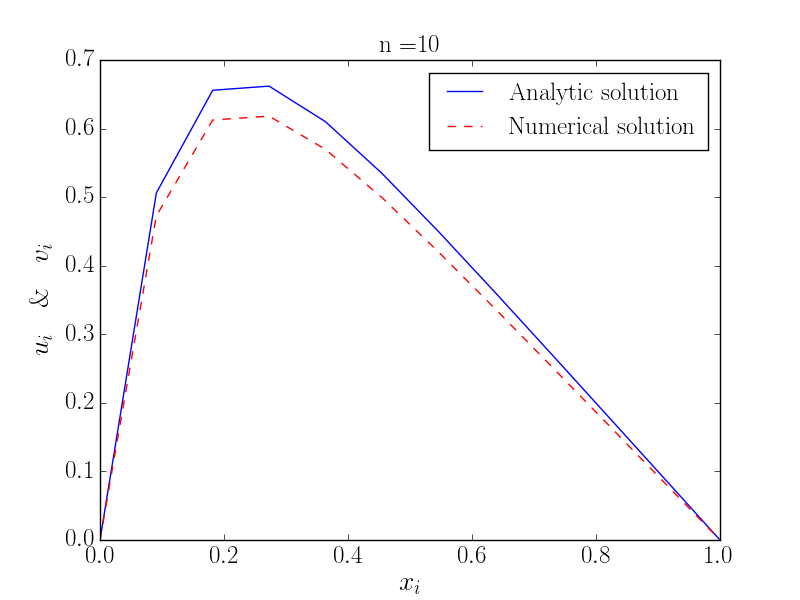
\includegraphics[width=0.9\linewidth]{figures/10.png}
  \caption{Numerical approximation of the tridiagonal matrix algorithm for $n=10$}
  \label{fig:n10}
\end{figure}

\begin{figure}[h]
  \centering
  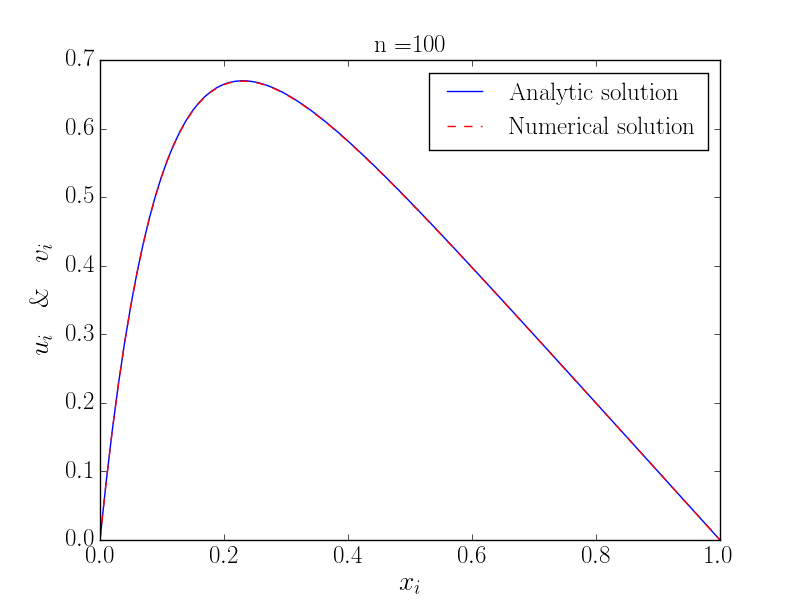
\includegraphics[width=0.9\linewidth]{figures/100.png}
  \caption{Numerical approximation of the tridiagonal matrix algorithm for $n=100$}
  \label{fig:n100}
\end{figure}

Figure \ref{fig:relerror} shows a plot of the maximum relative error of the
tridiagonal solver as a function of step size. One can see that the
relative error falls as the step size falls, but only to a certain
point. By decreasing the step size further the error increases, most
likely because of decreasing numerical precision because of the
computers difficulty in representing very small numbers.

\begin{figure}[h]
  \centering
  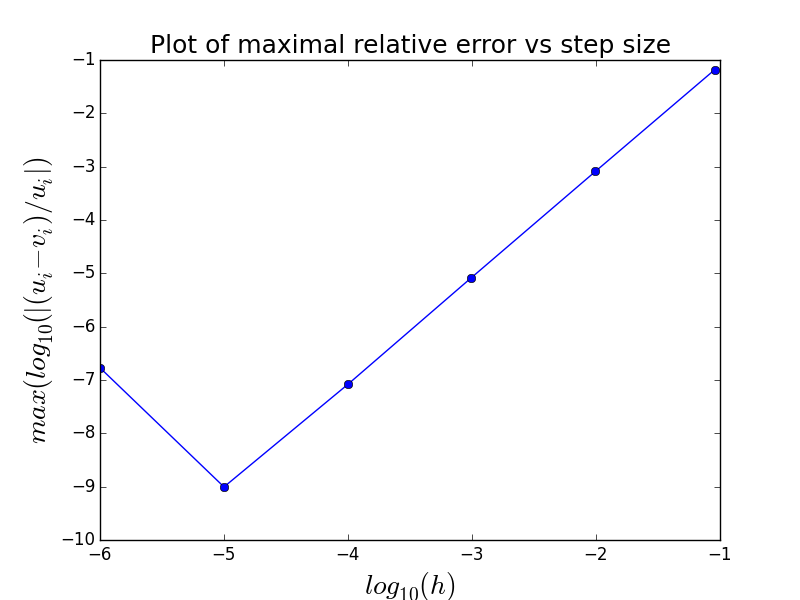
\includegraphics[width=0.9\linewidth]{figures/relerror.png}
  \caption{Plot of maximum relative error as a function of step size}
  \label{fig:relerror}
\end{figure}

\section{Discussion}
When choosing a suitible value for $n$, one must take into account both precision and speed. Our intuition tells us that a larger $n$ should result in a higher precision for the numerical derivative. We can conclude from figure \ref{fig:relerror} that this is only true up to a certain point, because of loss in numerical representation accuracy within the computer. An ideal n will be in the magnitude of $10^5$ which is equivalent to $h=10^-5$. Increasing this value will not increase run time dratically for the tridiagnoal matrix algorithm. Choosing $n=10^5$ gives us the ability to calculate with a high certainty of 5 decimals points and with low memory cost. 

By looking at the results one is led to believe that there are more reasons to prefer the tridiagonal matrix algorithm for this kind of problem. When using the LU decomposition method the short term memory is quickly filled with nothing but the matrix $A$. Choosing $n=10^5$ is equivalent to $8\times10^{10}$ bytes$=80$GB of memory! A brand new computer ships with around $8$ GB of memory today, which is a tenth of the space required. Obviously, this inhibits our ability to perform the calculation. 

\section{Conclusion}
As we have seen, there is significant advantage to fine-tuning and picking the correct algorithm before solving a problem numerically. We have experienced the restrictions in memory when computing, and have been made aware of the problem this poses when doing numerical calculations. The specialised tridiagonal matrix algorithm was able to solve the one-dimensional Poisson equation more than $20000$ times faster than the more general LU decomposition method. This can be explained by the fact that the LU decomposition method require $\mathcal{O}(\frac{2}{3}n^3)$ FLOPS while the specialized tridiagonal matrix algorithm will do with a meager $\mathcal{O}(8n)$ FLOPS.

\begin{thebibliography}{10}
  \bibitem{thomasalgo}{Thomas, L.H. (1949), \emph{Elliptic
        Problems in Linear Differential Equations over a
        Network}. Watson Sci. Comput. Lab Report, Columbia University,
      New York.}
    \bibitem{morten}{Hjorth-Jensen, M. (2015). \emph{Computational
        Physics - Lecture Notes 2015}. University of Oslo}
    \bibitem{golub}{Golub, G.H., van Loan, C.F. (1996). \emph{Matrix
          Computations} (3rd ed.), Baltimore: John Hopkins.}
\end{thebibliography}

\end{document}
